\documentclass[a4paper, 12pt,notitlepage]{article} % Use this for standard document

\usepackage{fontspec} % Need this to use Optima
\usepackage[left=0.9in,right=0.9in,top=1in,bottom=1in]{geometry} % Use this to control margins
\usepackage{amsthm,amsmath, amssymb} % provides numberwithin (and lots more)
\usepackage{lipsum}  % for sample text
\usepackage{mathtools} %put text over arrow

\setmainfont{Times New Roman} % Set main font here

% images:
\usepackage{graphicx}
\graphicspath{ {../Slides/Images/} }

%double spacing
\usepackage{setspace}

% extra spacing get rid of!
\usepackage[explicit]{titlesec}
\titlespacing*{\section}{0pt}{2pt}{2pt} % sections
\newenvironment{tightcenter}{% centers
	\setlength\topsep{2pt}
	\setlength\parskip{2pt}
	\singlespacing % ALSO: make single spaced
	\begin{center}
	}{%
	\end{center}
}
\setlength\intextsep{1.0\baselineskip plus 3pt minus 2 pt} % figures
\newenvironment{figurecenter}{% centers
	\setlength\topsep{-7pt}
	\setlength\parskip{-7pt}
	\singlespacing % ALSO: make single spaced
	\begin{center}
	}{%
	\end{center}
\vspace{-5pt}
}
\usepackage[font=small,skip=0pt]{caption} % captions


%colors\dfrac{num}{den}
\usepackage[usenames, dvipsnames]{color}

% Make counter for theorems/defns/examples
\newcounter{dummy}
\numberwithin{dummy}{subsection}
\numberwithin{dummy}{section}

% Declare theorems
\theoremstyle{named}
%\theoremstyle{definition}		% use to non-italicize theorem
\newtheorem{theorem}{Theorem}[dummy]
\newtheorem{definition}[theorem]{Definition}

\theoremstyle{definition}
\newtheorem{qustion}[theorem]{Question}

\theoremstyle{definition}
\newtheorem{exmple}[theorem]{Example}



% Make commands to keep number straight between sections & subsections
\renewcommand{\thetheorem}{%
	\ifnum\value{subsection}=0 
	\thesection% "no section"
	\else
	\thesubsection% at least within a section
	\fi%
	.\arabic{theorem}}

\renewcommand{\thedefinition}{%
	\ifnum\value{subsection}=0 
	\thesection% "no section"
	\else
	\thesubsection% at least within a section
	\fi%
	.\arabic{dummy}}

\renewcommand{\thequstion}{%
	\ifnum\value{subsection}=0 
	\thesection% "no section"
	\else
	\thesubsection% at least within a section
	\fi%
	.\arabic{dummy}}

% Allow for naming of thms/defns/examples
\makeatletter
\def\thmhead@plain#1#2#3{%
	\thmname{#1}\thmnumber{\@ifnotempty{#1}{ }\@upn{#2}}%
	\thmnote{. {\the\thm@notefont\textbf{\textit{#3}}}}}
\let\thmhead\thmhead@plain
\makeatother

% change spacing around thms/defns/examples
\makeatletter
\def\thm@space@setup{%
	\thm@preskip=\bigskipamount
	\thm@postskip=\thm@preskip % or whatever, if you don't want them to be equal
}
\makeatother

% Show "Section" before section numbers

\titleformat{\section}{ \normalfont\bfseries\centering}{}{0em}{Section \thesection.\ #1}
\titleformat{\subsection}{\normalfont\bfseries\centering}{}{0em}{\thesubsection.\ #1}




 % make sections appear on new pages and link
\usepackage{hyperref}
\let\stdsection\section
%\renewcommand\section{\cleardoublepage\stdsection}

% Indent options
\setlength\parindent{0.5in}
\usepackage{indentfirst}

% To center columns
\usepackage{array}
\newcolumntype{P}[1]{>{\centering\arraybackslash}m{#1} }

\usepackage{calc} % for extra height cells


\usepackage[shortlabels]{enumitem} % for no spacing between lists

\usepackage{framed} % for boxes

% make questions go in box
\usepackage{environ}
\NewEnviron{question}{\begin{framed}\vspace{-10pt}\begin{qustion}{\BODY}\end{qustion}\vspace{-10pt}\end{framed}}
\NewEnviron{example}{\renewcommand{\qedsymbol}{|\hspace{-1pt}|}\begin{exmple}{\BODY}\qed\end{exmple}}

% tabbing in tables
\usepackage{booktabs}% http://ctan.org/pkg/booktabs
\newcommand{\tabitem}{~~\llap{\textbullet}~~}

\usepackage{wrapfig} % to wrap text around figures



% title/table of contents
\makeatletter
\newcommand*{\toccontents}{\@starttoc{toc}}
\makeatother

% change spacing of \\ -> store as \nl
\newcommand{\nl}{\\[\bigskipamount]
	
	\vspace{-12pt}
}

% adjust title location on title page%
\usepackage{titling}
\renewcommand\maketitlehooka{\null\vspace{125pt}}
%\renewcommand\maketitlehookd{\vfill\null}

% make picture command
\newcommand{\pic}[2]{
	
	%\vspace{12pt}
	\centerline{\includegraphics[scale=#1]{#2}}
	%\vspace{12pt}
	
	
}
\usepackage{float} % for [H] option

% for complex tables
\usepackage{multirow}

% make symbols bold
\newcommand{\bld}[1]{\boldsymbol{#1}}

%for title
\usepackage{titling}

% for argmin
\usepackage{amsmath}
\DeclareMathOperator*{\argmin}{argmin} % thin space, limits underneath in displays

% endnotes
\usepackage{endnotes}
\renewcommand{\notesname}{Endnotes}

% bibliography spacing
\usepackage{natbib}
\setlength{\bibsep}{0.0pt}

% for headers
\usepackage{fancyhdr}
% remove bar
\fancyhf{} % sets both header and footer to nothing
\renewcommand{\headrulewidth}{0pt}

\begin{document}
	\setlength{\droptitle}{-15.5em}
	\title{\textbf{Uncovering Hidden Meaning in the \textit{De Re Publica}}\vspace{-2.5ex}}
	\author{{\Large \textbf{A Computational Analysis of the Text}}}
%	\date{\vspace{-1.8ex}\today}
\date{}
	
	\maketitle
	\vspace{-50pt}
	
	\doublespacing
	
	\thispagestyle{fancy}
	\cfoot{}
	\rhead{Marc E. Canby\\April 24, 2018\\Word Count: $1598$}
	
	For centuries, classical scholars have analyzed Latin texts simply by reading them, which has allowed scholars to decipher meaning, find patterns, and discover historical information. However, certain features of the text can be difficult $-$ and sometimes impossible $-$ to ascertain by studying them in this way: for example, a problem as basic as determining the average number of words in a sentence can be difficult for humans reading the text to solve. With the advent of high-speed computers in the last half-century, such problems are now tractable, opening the door to information about the text that was not previously available.
	
	In this paper, I will perform a computational analysis of Cicero's \textit{De Re Publica}. I will emphasize an analysis that is not attainable simply by reading the text. I will first explain how I obtained the text on the computer and perform a preliminary analysis. Then, I will investigate \textit{distributional word semantics}, which studies semantic relationships between words. Finally, I will perform \textit{sentence clustering}, which groups sentences based on their meaning. This paper is designed to be accessible to students of Latin without little to no math and computer science background.
	
	\pagestyle{myheadings}
	
	\section{Obtaining and Cleaning the Data}
	
	I choose to use the Python coding language\endnote{All of my code, as well as other information, can be found at \cite{code}.}, a popular choice for researchers in text analysis. I accessed a digital copy of the \textit{De Re Publica} from the \textit{Latin Library}, which is made up of sentences of the following form\endnote{I used the Classical Languages Toolkit (CLTK), a Python library with support for loading classical texts, performing morphological analyses, and running various algorithms \cite{cltk}.}:
	
	\begin{tightcenter}
	{\small \ttfamily ['nempe', 'ab', 'iis', 'qui', 'haec', 'disciplinis', 'informata', 'alia', 'moribus', 'confirmarunt', ',', 'sanxerunt', 'autem', 'alia', 'legibus', '.']} \cite[I.2]{drp}
	\end{tightcenter}

	\noindent I first cleaned several ``messy" elements of the raw text. For example, consider the beginning of the first sentence:
	
	\begin{tightcenter}
		{\small \ttfamily ['\&', 'lt', ';', 'im\&gt', ';', 'petu', 'liberavissent', ',', 'nec', ...]} \cite[I.1]{drp}
	\end{tightcenter}

\noindent	Clearly, left and right angle brackets ({\ttfamily <} and {\ttfamily >}) are encoded as {\ttfamily \&lt;} and {\ttfamily \&gt;} respectively; I amended these to their proper symbol before proceeding. English titles such as

	\begin{tightcenter}
		{\small \ttfamily [‘Cicero’, ‘The’, ‘Latin’, ‘Library’, ‘Classics’, ‘Page’]}
	\end{tightcenter}

\noindent also occurred in the text, which I removed before examining the data. Neglecting to clean the text in these ways could result in misleading conclusions.

\section{Exploratory Text Analysis}

I begin with an exploratory analysis. I first compare the size of the text to the average size among Cicero's philosophical treatises\endnote{I used the works that \textit{The Latin Library} deems to be Cicero's philosophical works for this analysis. A listing can be found at \cite{drp}.}:

\begin{figure}[H]
	\begin{figurecenter}
	\begin{tabular}{| c | c | c |}
		\hline
		 & \textit{De Re Publica}  &  Average across Cicero's Philosophy \\ \hline
		Number of characters & $109,777$  &  $136,893$ \\ \hline
		Number of words  & $20,067$  & $24,924$  \\ \hline
		Number of sentences & $820$  & $1,059$  \\
		\hline
	\end{tabular}\\
\caption{Size of Text}
\end{figurecenter}
\end{figure}


\noindent We see that the \textit{De Re Publica} is shorter than Cicero's average philosophy work. I also analyze the part-of-speech distribution\endnote{I used pre-built functionality from the CLTK to determine parts of speech; I did not code a part-of-speech tagger from scratch \cite{cltk}. I also used the {\ttfamily ggplot} package in the R coding language to produce these plots \cite{ggplot}.}:

\begin{figure}[H]
	\begin{figurecenter}
	\begin{minipage}{.5\textwidth}
		\centering
		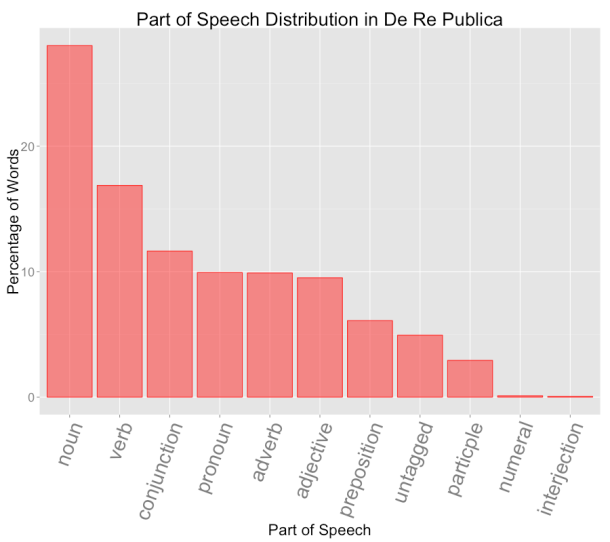
\includegraphics[scale=0.75]{image1.png}
	\end{minipage}%
	\begin{minipage}{.5\textwidth}
		\centering
		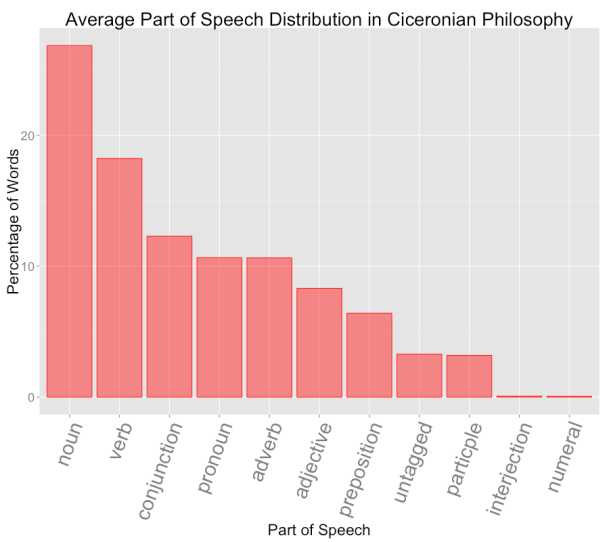
\includegraphics[scale=0.75]{image2.png}
	\end{minipage}
	\caption{Part-of-speech Distribution}
	\end{figurecenter}
\end{figure}

\noindent As expected, nouns and verbs are most common, followed by conjunctions. There does not appear to be a significant difference between the part-of-speech distributions of the \textit{De Re Publica} and Cicero's other philosophical works, which is a naive indicator that this text does not deviate greatly from Cicero's ``average" writing style.

\section{Distributional Word Semantics: Introduction}

After exploring the data, I investigate distributional word semantics, which examines semantic relationships between linguistic items (such as words and sentences) in a text corpus. The goal is to encode each item as a vector (series of numbers) and analyze the relationship among the vectors. Consider Figure \ref{iota} below:

\begin{figure}[H]
	\begin{figurecenter}
	\begin{minipage}{.5\textwidth}
		\centering
		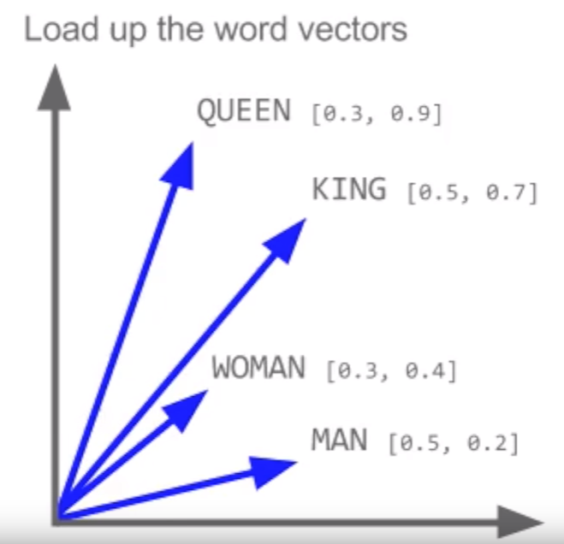
\includegraphics[scale=0.68]{image4.png}
	\end{minipage}%
	\begin{minipage}{.5\textwidth}
		\centering
		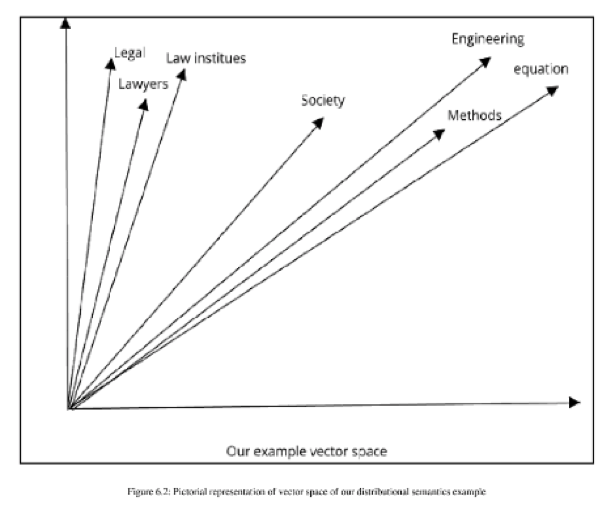
\includegraphics[scale=0.75]{image3.png}
	\end{minipage}
	\caption{Distributional Word Semantics \cite{kindqueen,pythonnlp}}
	\label{iota}
	\end{figurecenter}
\end{figure}

\noindent The left figure shows the relationship between the words ``king" and ``queen": {\ttfamily queen = king - man + woman}. The right figure shows what might happen if we perform this analysis on a group of legal and scientific articles: legal terms such as ``lawyers" and ``law institutes" occur in more similar contexts than scientific terms like ``engineering" and ``equation".

\section{Distributional Word Semantics: Word2Vec Algorithm}

To analyze distributional word semantics, I use the Word2Vec algorithm, which was invented by Google in 2013. Figure \ref{a} shows an overview of the algorithm \cite{pythonnlp, gensim}:

\begin{figure}[H]
	\begin{figurecenter}
	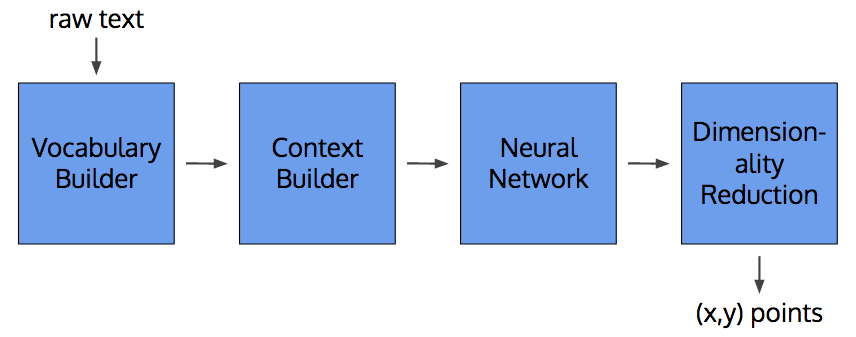
\includegraphics[scale=0.4]{image5.png}
	\caption{Overview of Word2Vec Algorithm}
	\label{a}
	\end{figurecenter}
\end{figure}

\noindent To illustrate how the algorithm works, I will show its effect on a single sentence:

\begin{tightcenter}
	{\small \ttfamily ['nempe', 'ab', 'iis', 'qui', 'haec', 'disciplinis', 'informata', 'alia', 'moribus', 'confirmarunt', ',', 'sanxerunt', 'autem', 'alia', 'legibus', '.']}
\end{tightcenter}

\noindent Since declension and conjugation generally do not alter the meaning of words, we use the \textit{base form}, or dictionary entry, of each word. We also remove \textit{stop words}, which are words like \textit{et} and \textit{sum} that add little additional meaning to sentences. Retaining these words tends to mislead the algorithm. We would transform the example sentence as follows\endnote{Algorithms to identify stop words and \textit{lemmatize} words (find the base forms of inflected words) are provided by the CLTK \cite{cltk}.}:

%First, we map each word to its \textit{base form}, or dictionary form. This allows declined and conjugated forms of a word to be treated equivalently, as there is essentially no semantic difference between words like \textit{urbe} and \textit{urbis}. The Vocabulary Builder also removes \textit{stop words}, which are words like \textit{et} and \textit{sum} that provide little additional meaning to sentences (these are highlighted in red below). Retaining these words tends to mislead the algorithm. Thus, we would transform the example sentence as follows:

\begin{tightcenter}
	{\small \ttfamily ['nempe', 'ab', 'iis', 'qui', 'haec', 'disciplinis', 'informata', 'alia', 'moribus', 'confirmarunt', ',', 'sanxerunt', 'autem', 'alia', 'legibus', '.']}\\
	\vspace{3pt}
	$\big \Downarrow$
	\vspace{3pt}\\
	{\small \ttfamily ['nempe', {\color{red}'ab'}, {\color{red}'is'}, {\color{red}'qui'}, {\color{red}'hic'}, 'disciplina', 'informo', 'alius2', 'mos', 'confirmo', 'sancio', {\color{red}'autem'}, 'alius2', 'lex']}\\
	\vspace{3pt}
	$\big \Downarrow$
	\vspace{3pt}\\
	{\small \ttfamily ['nempe', 'disciplina', 'informo', 'alius2', 'mos', 'confirmo', 'sancio', 'alius2', 'lex']}
	
\end{tightcenter}

Next, we build \textit{context pairs} for each word in the text: this represents every word by the words around it. Figure \ref{beta} shows the context pairs for our sample sentence (note that {\ttfamily '----'} denotes the beginning and end of a sentence):

\begin{figure}[H]
	\begin{figurecenter}
		\begin{tabular}{| c | c |}
			\hline
			{\ttfamily ('----','disciplina')} $\rightarrow$ {\ttfamily 'nempe'} & {\ttfamily ('mos','sancio')} $\rightarrow$ {\ttfamily 'confirmo'} \\ \hline
			{\ttfamily ('nempe','informo')} $\rightarrow$ {\ttfamily 'disciplina'} & {\ttfamily ('confirmo','alius2')} $\rightarrow$ {\ttfamily 'sancio'}   \\ \hline
			{\ttfamily ('disciplina','alius2')} $\rightarrow$ {\ttfamily 'informo'} & {\ttfamily ('sancio','lex')} $\rightarrow$ {\ttfamily 'alius2'}   \\ \hline
			{\ttfamily ('informo','mos')} $\rightarrow$ {\ttfamily 'alius2'} & {\ttfamily ('alius2','----')} $\rightarrow$ {\ttfamily 'lex'}    \\ \hline
			{\ttfamily ('alius2','confirmo')} $\rightarrow$ {\ttfamily 'mos'} &    \\ \hline
		\end{tabular}\\
		\caption{Context Builder Example}
		\label{beta}
	\end{figurecenter}
\end{figure}

\noindent The entry {\ttfamily ('nempe','informo')} $\rightarrow$ {\ttfamily 'disciplina'}, for example, indicates that the word {\ttfamily 'disciplina'} can be found between words {\ttfamily 'nempe'} and {\ttfamily 'informo'}. %Thus, this is a way to represent context in the text.

The final step of the algorithm generates a vector for each word. The idea is that words with similar vectors appear in similar contexts. The details of this step are highly complex; Figure \ref{gamma} provides an overview:

\begin{figure}[H]
	\begin{figurecenter}
	\begin{minipage}{.6\textwidth}
		\centering
		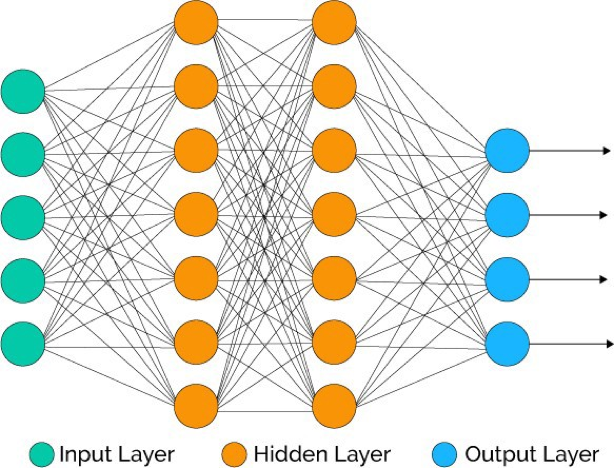
\includegraphics[scale=0.68]{image6.png}
	\end{minipage}%
	\begin{minipage}{.4\textwidth}
		\centering
		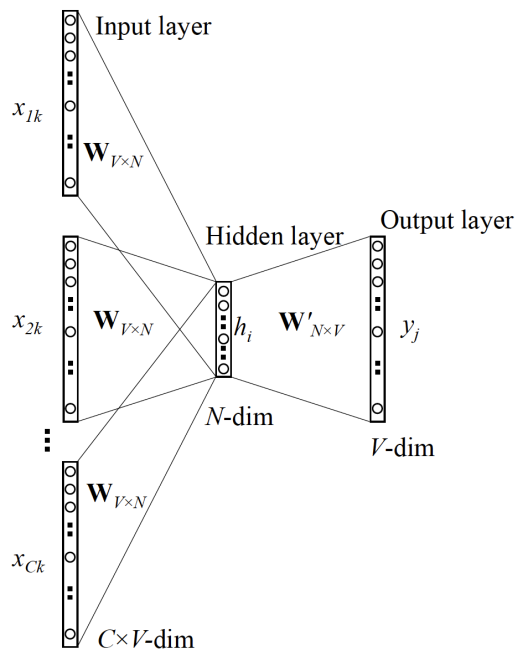
\includegraphics[scale=0.68]{image7.png}
	\end{minipage}
	\caption{Neural Network in Word2Vec \cite{towards, cbow}}
	\label{gamma}
	\end{figurecenter}
\end{figure}

\noindent The left figure illustrates a generic \textit{neural network}; each circle is a neuron and each line connects neurons. This attempts to model the human brain: humans perceive multidimensional input (represented by the green circles) and make an educated decision about their perception (represented by one of the blue circles). The right image shows the neural network setup for Word2Vec; each rectangle on the input layer represents a context word, and each circle on the output layer represents a unique word in the text\endnote{This is called the Continuous Bag of Words (CBOW) architecture; another common architecture for Word2Vec is the Skip-gram. A discussion of the difference between the architectures can be found at \cite{pythonnlp}. I obtained better results on the CBOW architecture.}. By observing context pairs, the network attempts to maximize the probability of predicting the correct word for a given context. Once optimized, the matrix $\bld{W}_{V \times N}$ contains the vectors for each word.

\section{Distributional Word Semantics: Results}

We now present the results of running this algorithm on the \textit{De Re Publica}. After reducing the size of the vectors to two dimensions\endnote{I used the $t$-Distributed Stochastic Neighbor Embedding (t-SNE) algorithm for dimensionality reduction. I also attempted Principle Component Analysis (PCA) and Independent Component Analysis (ICA), but had best results with $t$-SNE \cite{dimred}.}, we obtain the plot shown in Figure \ref{delta}:

\begin{figure}[H]
	\begin{figurecenter}
	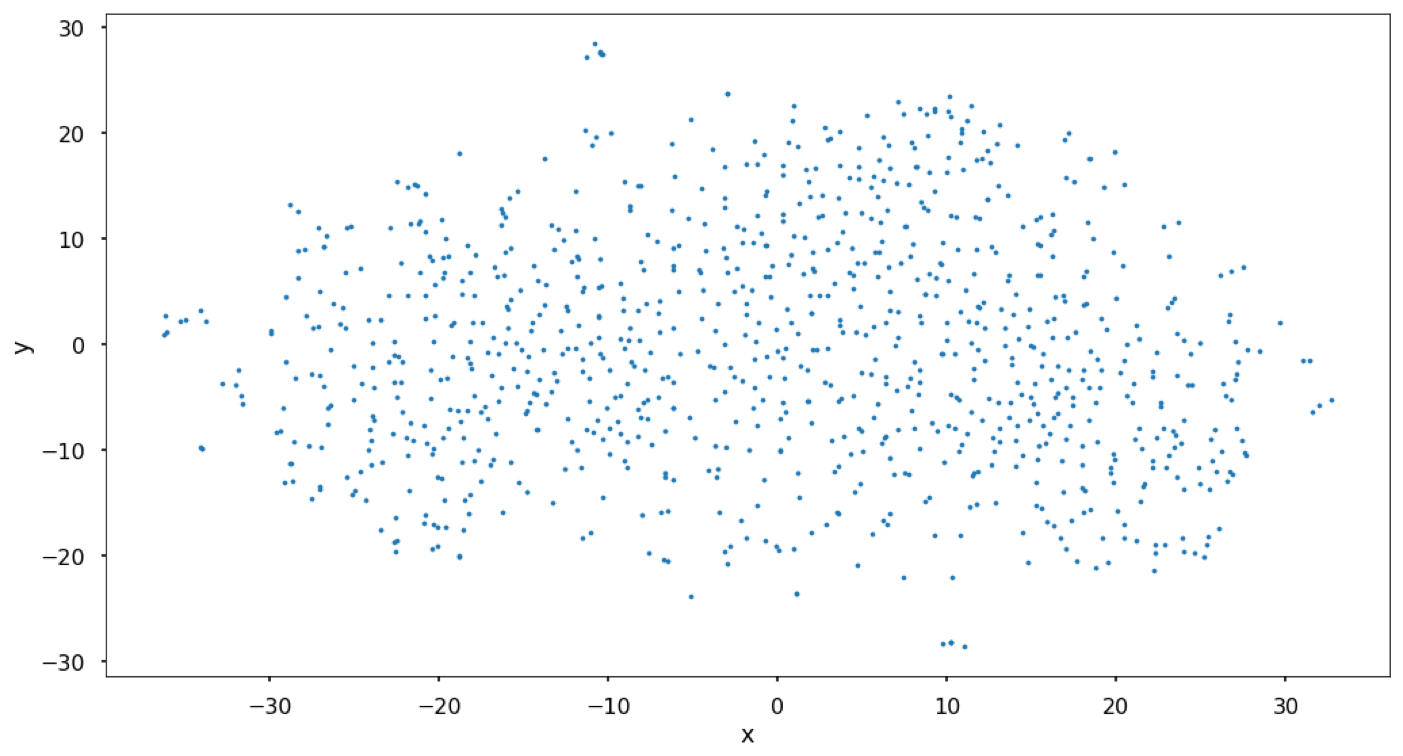
\includegraphics[scale=0.7]{image8.png}
	\caption{Word2Vec Results on the \textit{De Re Publica}}
	\label{delta}
	\end{figurecenter}
\end{figure}

\noindent Each point signifies a word, and nearby points represent words used in similar contexts. It is hard to ascertain much information from this figure, so we examine zoomed-in sections:

\begin{figure}[H]
	\begin{figurecenter}
	\begin{minipage}{.5\textwidth}
		\centering
		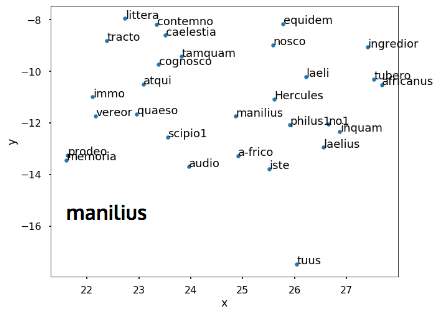
\includegraphics[scale=0.55]{image9.png}
	\end{minipage}%
	\begin{minipage}{.5\textwidth}
		\centering
		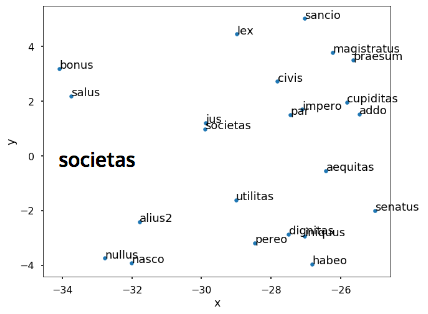
\includegraphics[scale=0.55]{image10.png}
	\end{minipage}
\begin{minipage}{.5\textwidth}
	\centering
	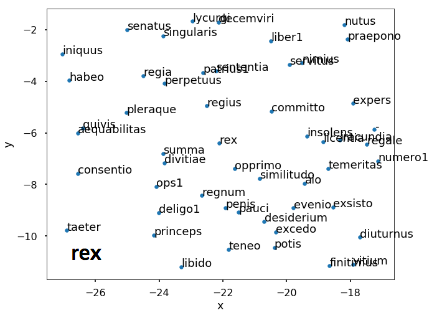
\includegraphics[scale=0.55]{image11.png}
\end{minipage}%
\begin{minipage}{.5\textwidth}
	\centering
	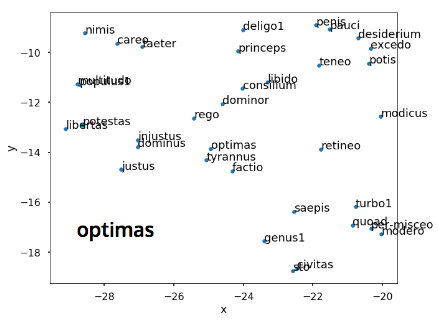
\includegraphics[scale=0.55]{image12.png}
\end{minipage}
	\caption{Zoomed Word2Vec Results on the \textit{De Re Publica}}
	\end{figurecenter}
\end{figure}

\noindent We see that Cicero uses names like \textit{Manilius}, \textit{Scipio} and \textit{Philus} in similar contexts, which makes sense since these are often the subjects of speaking verbs. Similarly, words like \textit{rex}, \textit{opprimo}, and \textit{regnum} appear near each other, which all relate to monarchical rule. An examination of the plots of \textit{societas} and \textit{optimas} shows similar patterns. Thus, this technique allows us to see patterns in Cicero's writing that are not necessarily evident when we read the text.

\section{Sentence Clustering: $\bld{K}$-Means Algorithm}

Next, I cluster sentences into $K$ groups with the classic $K$-means algorithm. Figure \ref{epsilon} provides an overview \cite{doccluster, pythonnlp}:

%Next, I investigate \textit{sentence clustering}, which is the grouping of sentences into $K$ categories based on meaning. A classic algorithm for doing this is $K$-means; Figure \ref{epsilon} gives an overview:

\begin{figure}[H]
	\begin{figurecenter}
	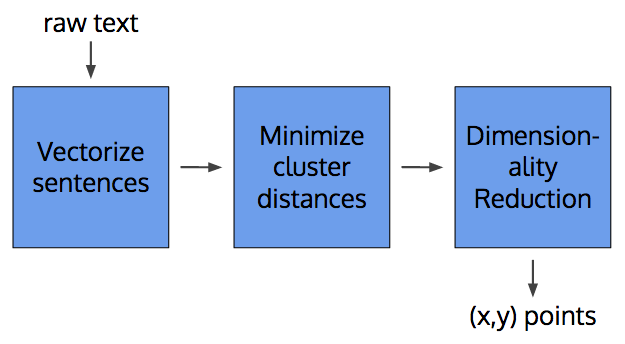
\includegraphics[scale=0.4]{image13.png}
	\caption{Overview of $K$-Means Algorithm}
	\label{epsilon}
	\end{figurecenter}
\end{figure}

We first represent sentences as vectors; the distance between vectors will indicate sentence similarity. I use the \textit{Term-Frequency-Inverse-Document-Frequency} representation, which encodes each sentence as a vector with length equal to the number of unique words in the text. The $i$th element of a sentence's vector denotes how many times the $i$th vocabulary term appears in that sentence. Since using pure counts would inevitably make longer sentences have larger entries, we normalize each sentence by its length, creating \textit{term frequencies}. The result is demonstrated on two sample sentences below (as before, I use base forms and remove stop words):

%First, we represent sentences as vectors, which will allow us to compute ``distances" between them; distance is an indicator of sentence similarity. I choose the \textit{Term-Frequency-Inverse-Document-Frequency} (TFIDF) representation. This encodes each sentence as a vector with length equal to the number of unique words in the text. The $i$th element of a sentence's vector indicates how many times the $i$th vocabulary term appears in the sentence. Since using pure counts would inevitably make longer sentences have larger entries, we normalalize each sentence by its length, creating \textit{term frequencies}. The result is demonstrated on two sample sentences below (as before, I map each word to its base form and remove stop words):

\begin{tightcenter}
	{\small \ttfamily ['nempe', 'disciplina', 'informo', 'alius2', 'mos', 'confirmo', 'sancio', 'alius2', 'lex']}\\{\ttfamily \small ['oratio', 'ex-quaero', 'antepono', 'benus', 'constituo', 'civitas', 'publicus', 'jus', 'mos']} \cite[I.2]{drp}\\
	\vspace{3pt}
	$\big \Downarrow$
	\vspace{3pt}\\
	{\small \ttfamily [1,1,1,2,1,1,1,1,0,0,0,0,0,0,0,0]}\\{\ttfamily \small [0,0,0,0,1,0,0,0,1,1,1,1,1,1,1,1]}\\
	\vspace{3pt}
	$\big \Downarrow$
	\vspace{3pt}\\
	{\small \ttfamily [1/9,1/9,1/9,2/9,1/9,1/9,1/9,1/9,0,0,0,0,0,0,0,0]}\\{\ttfamily \small
		[0,0,0,0,1/9,0,0,0,1/9,1/9,1/9,1/9,1/9,1/9,1/9,1/9]
	}
	
\end{tightcenter}

\noindent The idea behind \textit{inverse document frequencies} penalizes the values of words that appear in many sentences; for example, a word that appears in every sentence will be unlikely to help distinguish sentences, and its value would be set to $0$ in every sentence. The mathematics behind this is omitted\endnote{Readers interested in TFIDF vectors can find more information at \cite{pythonnlp}.}.

Next, we use the $K$-means algorithm to assign a group to each sentence. The algorithm is described below:

\begin{enumerate}
	\itemsep 0em
	\item Assign $K$ centroids (vectors) randomly, corresponding to the center of each group.
	\item For each sentence, calculate the distance to each centroid, and assign the sentence to the group with the nearest centroid.
	\item Calculate new centroids based on the sentence assignments, and repeat until convergence.
\end{enumerate}

\section{Sentence Clustering: Results}

After running this algorithm on the \textit{De Re Publica} and reducing the dimensionality of the vectors, we get the following results:

\begin{figure}[H]
	\begin{figurecenter}
	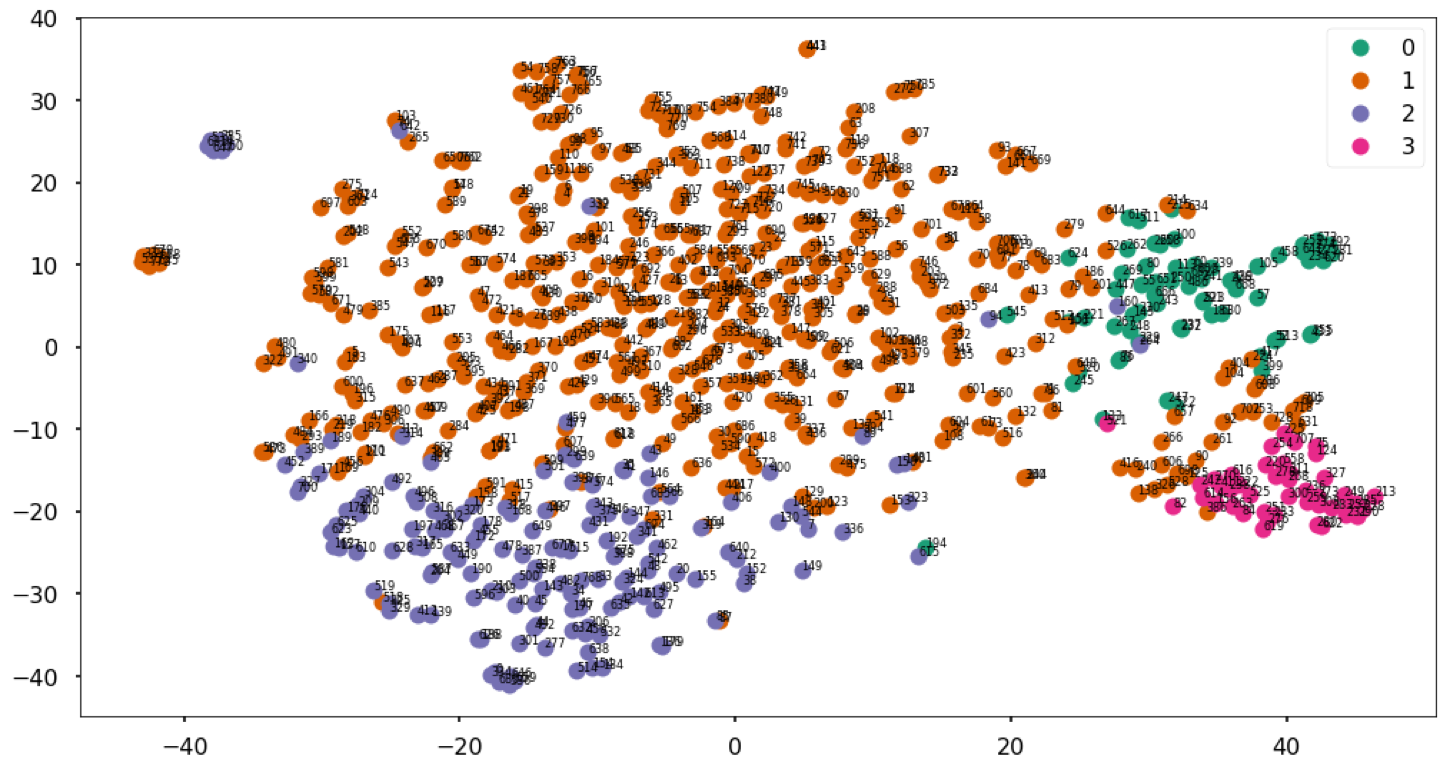
\includegraphics[scale=0.7]{image14.png}
	\caption{Sentence Clustering Results on the \textit{De Re Publica}}
	\label{zeta}
	\end{figurecenter}
\end{figure}

\noindent Each point in Figure \ref{zeta} represents a sentence, and its color indicates to which of four groups it belongs. We see a clear separation between groups, which means the sentences truly belong to distinct categories.

Figure \ref{eta} shows the words that are most indicative of group membership, and Figure \ref{theta} shows three sample sentences from each group\endnote{Three sentences were selected at random from each group.}:

\begin{figure}[H]
	\begin{figurecenter}
		\begin{tabular}{| c | c | c | c |}
			\hline
			\textbf{Cluster 0} & \textbf{Cluster 1} &\textbf{Cluster 2} &\textbf{Cluster 3}  \\ \hline
			{\ttfamily  scipio1} & {\ttfamily homo}  &  {\ttfamily res} & {\ttfamily laelius} \\ \hline
			{\ttfamily reor} & {\ttfamily magnus}  &  {\ttfamily publicus} & {\ttfamily inquam} \\ \hline
			{\ttfamily inquam} & {\ttfamily eo1}  &  {\ttfamily populus1} & {\ttfamily verus} \\ \hline
			{\ttfamily probo} & {\ttfamily verus}  &  {\ttfamily redeo} & {\ttfamily minimus} \\ \hline
			{\ttfamily quaero} & {\ttfamily civitas}  &  {\ttfamily bonus} & {\ttfamily philus1} \\ \hline
			{\ttfamily magnus} & {\ttfamily fero}  &  {\ttfamily genus1} & {\ttfamily nosco} \\ \hline
			{\ttfamily censeo1} & {\ttfamily bonus}  &  {\ttfamily magnus} & {\ttfamily no1} \\ \hline
			{\ttfamily sentio} & {\ttfamily ito}  &  {\ttfamily sto} & {\ttfamily saepis} \\ \hline
			{\ttfamily rex} & {\ttfamily facio}  &  {\ttfamily eo1} & {\ttfamily probe} \\ \hline
			{\ttfamily verus} & {\ttfamily populus1}  &  {\ttfamily cicero} & {\ttfamily sentio} \\ \hline
		\end{tabular}\\
		\caption{Most Indicative Words by Cluster}
		\label{eta}
	\end{figurecenter}
\end{figure}

\begin{figure}[H]
	\begin{figurecenter}
		\small
			\begin{tabular}{|c|m{14cm}|}
				\hline
				\textbf{Cluster} & \multicolumn{1}{|c|}{\textbf{Sentences}}   \\ \hline
				 {\textbf{0}} &  \begin{itemize}[leftmargin=*] \vspace{-0.3cm} \itemsep -0.15cm \item (scipio) `et talis est quaeque res publica, qualis eius aut natura aut voluntas qui illam regit \cite[I.4]{drp}. \item (scipio) `quid? \cite[I.61]{drp} \item (scipio) `ille vero, et magna quidem cum \cite[I.23]{drp} \vspace{-0.4cm} \end{itemize}  \\ 
				 \hline
				{\textbf{1}} &  \begin{itemize}[leftmargin=*] \vspace{-0.3cm} \itemsep -0.15cm \item tu enim quam celebritatem sermonis hominum aut quam expetendam consequi gloriam potes? \cite[VI.20]{drp} \item itaque ut tum carere rege, sic pulso tarquinio nomen regis audire non poterat. \cite[II.52]{drp} \item quare et tibi, publi, et piis omnibus retinendus animus est in custodia corporis nec iniussu eius, a quo ille est vobis datus, ex hominum vita migrandum est, ne munus humanum assignatum a deo defugisse videamini. \cite[VI.15]{drp} \vspace{-0.4cm} \end{itemize}  \\ 
				\hline
				{\textbf{2}} &  \begin{itemize}[leftmargin=*] \vspace{-0.3cm} \itemsep -0.15cm \item quod ita cum sit, ex tritus primis generibus longe praestat mea sententia regium, regio autem ipsi praestabit id quod erit aequatum et temperatum ex tribus primis rerum publicarum modis. \cite[I.69]{drp} \item sed quoniam de re publica loquimur, sunt que inlustriora quae publice fiunt, quoniamque eadem est ratio iuris in utroque, de populi sapientia dicendum puto, et ut iam omittam alios: noster hic populus, quem africanus hesterno sermone a stirpe repetivit, cuius imperio iam orbis terrae tenetur, iustitia an sapientia est e minimo omnium maximus factus? \cite[III.24]{drp} \item hoc errore vulgi cum rem publicam opes paucorum, non virtutes tenere coeperunt, nomen illi principes optimatium mordicus tenent, re autem carent eo nomine. \cite[I.51]{drp} \vspace{-0.4cm} \end{itemize}  \\ 
				\hline
				{\textbf{3}} &  \begin{itemize}[leftmargin=*] \vspace{-0.3cm} \itemsep -0.15cm \item (laelius) `adducor,' inquit, 'et prope modum adsentior.' \cite[I.61]{drp} \item tum laelius: `ego vero istud ipsum genus orationis quod polliceris expecto.' \cite[I.38]{drp} \item (laelius) `ista vero' inquit `adulta vix'. \cite[I.58]{drp} \vspace{-0.4cm} \end{itemize}  \\ 
				\hline
			\end{tabular}
			\caption{Sentences by Cluster}
			\label{theta}

	\end{figurecenter}
\end{figure}

\noindent Clusters 0 and 3 clearly contain small sentences spoken by Scipio and Laelius respectively. It is harder to tell the difference between Clusters 1 and 2. Therefore, I searched for patterns in clustering across the entire text\endnote{The text with each sentence highlighted by group membership can be found at \cite{code}.}: practically all of the passages about astronomy belong to Cluster 1, and quotes about forms of government are equally divided between Clusters 1 and 2. I should note that we do not necessarily expect to see obvious differences in the clusters; the fact that similar topics are assigned to different groups suggests that Cicero $-$ perhaps subconsciously $-$ alters his vocabulary in sentences about the same subject. This is an interesting insight about the text that may be hard to see when reading it.

\section{Challenges and Conclusions}

Despite finding interesting results, I faced many challenges. For one, there has been very little research on computational analysis of ancient texts; most research has focused on modern languages. While the algorithms are not language-specific, results can vary widely on languages with different structures. For example, Latin, unlike English, is highly inflected, which means that its meaning is largely dependent on word endings as opposed to syntax. Thus, algorithms that rely on syntax, like Word2Vec, tend to perform worse on Latin than on English; consequently, I adjusted the algorithm's parameters to accommodate freer syntax. The $K$-means clustering algorithm, on the other hand, relies only on vocabulary that appears in each sentence, rendering it immune to syntactic issues. Thus, it is important to understand the underlying structure of the language when computationally analyzing text.

 In my research, I ran over a dozen algorithms, examining topics such as keyword extraction, summarization, and text generation; further analyses could explore sentiment analysis and comparisons to other Latin authors. I chose to present distributional word semantics and text clustering because I feel that these results are not obvious from reading the text. Performing a computational analysis can give us a fresh perspective on a work that is over 2000 years old, offering us a view into Cicero's mind that we have not seen before.

\pagebreak

\setcounter{section}{\thesection + 1}
\def\enotesize{\normalsize} 
\theendnotes

\pagebreak

\setcounter{section}{\thesection + 1}

\bibliographystyle{plain}
\bibliography{bibliography}

%	
%	\bibitem{code}
%	i
	
	
	

	
\end{document}
